\documentclass{ximera}

\title{Unit 1}

\begin{document}

\begin{abstract}
$A\mathbf{x} = b$ and the four subspaces.
\end{abstract}
\maketitle

The big picture of linear algebra, four fundamental subspaces:
\begin{image}
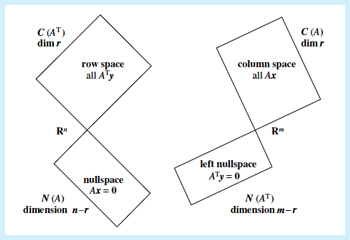
\includegraphics{Unit_1_WIDE.jpg}
\end{image}


Mathematics is a tool for describing the world around us. Linear
equations give some of the simplest descriptions, and systems of
linear equations are made by combining several descriptions.


In this unit we write systems of linear equations in the matrix form
$A\mathbf{x} = \mathbf{b}$. We explore how the properties of $A$ and
$\mathbf{b}$ determine the solutions $\mathbf{x}$ (if any exist) and
pay particular attention to the solutions to $A\mathbf{x} =
\mathbf{0}$. For a given matrix $A$ we ask which $\mathbf{b}$ can be
written in the form $A\mathbf{x}$.

\end{document}

